\section{Test-circuit validation: 8-bit parity checker}\label{sec:circuit}

\subsection{Circuit and SPICE reference}
The 8-bit parity checker outputs $1$ when an odd number of its eight inputs is $1$. No netlist is prescribed, so it was designed as a balanced tree of
seven XOR2 cells (four, two and one per level). Each XOR2 is the classic four-NAND2 realisation
\[
  n_1=\overline{a\,b},\qquad n_2=\overline{a\,n_1},\qquad n_3=\overline{b\,n_1},\qquad y=\overline{n_2\,n_3},
\]
so the circuit consists of 28 NAND2 gates (112 transistors, NAND2 sizing of \cref{sec:gates}) and every gate maps onto one of the four NAND2 input
cases of Part~B. The eight primary inputs are ideal sources at exactly $0$ or $\Vdd$ and the ground rail contains a 0\,V current probe, as in the
gate netlists (example netlists: \texttt{data/netlists/circuit/}).

The complete transistor-level netlist was simulated for all $2^8=256$ input vectors at the same 200 corners as the gates, i.e.\ $51{,}200$ SPICE runs,
each cross-checked as in \cref{sec:gates}. All runs converged with the mandated options, the cross-check agreed everywhere, and the output was at the
correct logic rail in every run, which confirms that the netlist implements the parity function.

\subsection{Hierarchical ML prediction}
For each input vector the logic value at the inputs of each of the 28 gates is found by logic propagation through the tree. The Part~B gate model of
that input combination, evaluated at the same corner, gives each gate's leakage, and the 28 gate leakages are summed
(\texttt{src/dvdml/circuit.py}, \texttt{scripts/09\_circuit\_ml.py}). As prescribed, this assumes that every gate input sits exactly at $0$ or $\Vdd$
and ignores loading between gates. The gate models in turn use only the four transistor models.

\subsection{Results}
\begin{table}[H]
\centering
{\small
\begin{adjustbox}{max width=\linewidth}
\begin{tabular}{lrrrrrrrr}
\toprule
input vectors & runs & SPICE median [A] & ML median [A] & bias & median err & P95 err & max err & mean acc. \\
\midrule
all 51,200 runs & 51200 & $2.87\times10^{-9}$ & $2.87\times10^{-9}$ & 0.14\% & 0.19\% & 0.79\% & 1.63\% & 99.73\% \\
0 ones in input & 200 & $3.33\times10^{-9}$ & $3.33\times10^{-9}$ & 0.14\% & 0.19\% & 0.74\% & 1.04\% & 99.75\% \\
1 ones in input & 1600 & $3.19\times10^{-9}$ & $3.19\times10^{-9}$ & 0.15\% & 0.19\% & 0.74\% & 1.09\% & 99.75\% \\
2 ones in input & 5600 & $3.10\times10^{-9}$ & $3.10\times10^{-9}$ & 0.14\% & 0.19\% & 0.76\% & 1.27\% & 99.74\% \\
3 ones in input & 11200 & $2.97\times10^{-9}$ & $2.97\times10^{-9}$ & 0.14\% & 0.19\% & 0.77\% & 1.29\% & 99.74\% \\
4 ones in input & 14000 & $2.90\times10^{-9}$ & $2.89\times10^{-9}$ & 0.14\% & 0.19\% & 0.79\% & 1.43\% & 99.73\% \\
5 ones in input & 11200 & $2.80\times10^{-9}$ & $2.80\times10^{-9}$ & 0.14\% & 0.19\% & 0.79\% & 1.45\% & 99.73\% \\
6 ones in input & 5600 & $2.74\times10^{-9}$ & $2.74\times10^{-9}$ & 0.13\% & 0.20\% & 0.80\% & 1.58\% & 99.72\% \\
7 ones in input & 1600 & $2.74\times10^{-9}$ & $2.74\times10^{-9}$ & 0.13\% & 0.20\% & 0.79\% & 1.55\% & 99.72\% \\
8 ones in input & 200 & $2.83\times10^{-9}$ & $2.84\times10^{-9}$ & 0.13\% & 0.20\% & 0.82\% & 1.63\% & 99.72\% \\
\bottomrule
\end{tabular}
\end{adjustbox}
}
\caption{Test-circuit results (8-bit parity checker, 256 input vectors $\times$ 200 corners): all runs, and grouped by the number of ones in the input vector.}
\label{tab:circuit}
\end{table}


\begin{table}[H]
\centering
{\small
\begin{adjustbox}{max width=\linewidth}
\begin{tabular}{lrrrrr}
\toprule
comparison & bias & median err & P95 err & max err & mean accuracy \\
\midrule
hierarchical ML vs circuit SPICE & 0.14\% & 0.19\% & 0.79\% & 1.63\% & 99.73\% \\
sum of isolated-gate SPICE vs circuit SPICE (loading only) & 0.00\% & 0.00\% & 0.01\% & 0.03\% & 100.00\% \\
\bottomrule
\end{tabular}
\end{adjustbox}
}
\caption{Source of the circuit-level error: ML prediction versus the error caused by ignoring loading between gates.}
\label{tab:cdecomp}
\end{table}



\begin{figure}[!htbp]\centering
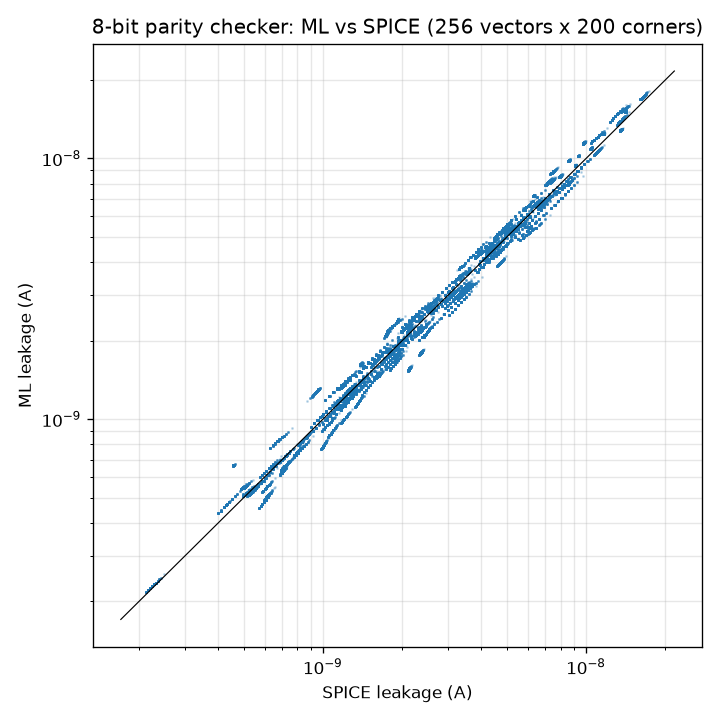
\includegraphics[width=.62\textwidth]{circuit_parity.png}
\caption{ML versus SPICE leakage of the 8-bit parity checker, all 51{,}200 runs (256 vectors $\times$ 200 corners), log axes.}\label{fig:cparity}
\end{figure}

Over all 51{,}200 runs the \textbf{mean accuracy is 99.73\,\%}: median error 0.19\,\%, P95 0.79\,\%, largest error 1.6\,\%, bias $+0.14$\,\%. The
accuracy does not depend on the input vector (99.72--99.75\,\% for zero to eight ones in the input).

\paragraph{Comparison with the gate level.} The assignment expects the circuit to be somewhat less accurate than the gates, because the composition
ignores loading. Here the circuit is as accurate as the gates (median 0.19\,\% at both levels), and its P95 and maximum errors are even lower
(0.79\,\% vs 1.2\,\%, 1.6\,\% vs 5.7\,\%). \Cref{tab:cdecomp} explains why: for rail-to-rail inputs, the sum of the SPICE leakages of the 28
\emph{isolated} gates reproduces the SPICE leakage of the complete circuit to within $10^{-4}$ (mean accuracy 99.996\,\%), so neglecting the loading
between gates costs essentially nothing and the circuit error is the error of the gate models. The circuit uses only NAND2 gates, which are the most
accurate gate type (\cref{tab:bygate}), and summing 28 gate leakages averages part of their random errors, which narrows the tails. The errors do not
average out completely, because all gates of one evaluation share the same corner and therefore the same systematic part of the model error
(\cref{sec:errors}).
